\section{Theorie}
\label{sec:Theorie}
Frequenzen im Bereich von $20 \si{\kilo\hertz}$ bis $1 \si{\giga\hertz}$ werden Ultraschall genannt.
Ultraschall kann mit piezoelektrischen Kristallen in einem elektrischen Wechselfeld erzeugt werden, die
Kristalle werden zum Schwingen angeregt, wenn eine polare Achse in Richtung des elekktrischen Feldes zeigt.
Im Falle der Resonanz können große Schwingungen erzeugt werden. Ebenso dienen die Kristalle als Empfänger von Ultraschallwellen.
Bei Messungen mit dem Ultraschall wird der Doppler-Effekt ausgenutzt, dieser beschreibt die Veränderung der
Frequenz, die auftritt bei relativer Bewegung von einem Sender und einem Empfänger.
Die Ultrasschallfrequenz $\nu_0$ wird verschoben zu:
\begin{align}
 \Delta \nu =2\nu_0 \frac{v}{c}(\cos{\alpha}),\label{eqn:deltav}
\end{align}
wenn die Ultraschallwelle auf ein bewegtes Objekt trifft zum Beispiel auf einen Blutkörper wie in Abbildung \ref{fig:1} zusehen.
Die Größe $c$ ist die Schallgeschwindigkeit, $\nu_0$ die Frequenz des Ultraschall-Generators und $\alpha$ der Winkel
zwischen der Geschwindigkeit und der Wellennormalen.
\begin{figure}
  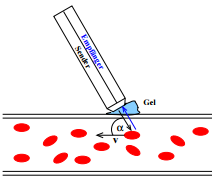
\includegraphics[width=0.7\textwidth]{Unbenannt1.png}
  \centering
  \caption{Darstellung der Winkelbeziehung zwischen Sender und Geschwindigkeitsvektor.\cite{sample} }
  \label{fig:1}
\end{figure}
